%!TEX program=xelatex
% 注意事项:编译两次,以确保目录、页码完整显示
% 华东师范大学软件工程学院课程报告
% https://github.com/Shichien/ECNU-LateX-Template
% Author - 10235101526

\def\allfiles{}

\documentclass[14pt,a4paper,UTF8,twoside]{article}

% Title Page ————————————————————————————————————————
\usepackage{titlesec}
\usepackage{setspace}

% Formatting Packages ——————————————————————————————————————
\usepackage{multicol}
\usepackage{multirow}
\usepackage{enumitem}
\usepackage{indentfirst}

% Math & Physics Packages ————————————————————————————
\usepackage{amsmath, amsthm, amsfonts, amssymb}
\usepackage{physics}
\usepackage{cancel}
\usepackage{nicefrac}
\usepackage{unicode-math} % 允许数学公式使用特定字体
\usepackage{mdframed}
\usepackage{forest}

% Image-related Packages —————————————————————————————
\usepackage{float} % 浮动体环境
\usepackage{subcaption} % 子图包
\usepackage{pgfgantt}
\usepackage{graphics, graphicx}
\usepackage{tikz, tikz-qtree}
\usetikzlibrary{arrows.meta, positioning, fit, shapes}
\usetikzlibrary{shapes.geometric}
\tikzstyle{node_style} = [rectangle, rounded corners, draw, align=center, text width=3cm, minimum height=0.65cm]
\tikzstyle{arrow_style} = [thick, ->, >=stealth]

\usepackage{pgfplots}
\pgfplotsset{compat=1.18}
\usepackage{xcolor}
\usepackage{fourier-orns}
\usepackage{lipsum}

% Colour Palette ——————————————————————————————————————
\definecolor{merah}{HTML}{F4564E}
\definecolor{merahtua}{HTML}{89313E}
\definecolor{biru}{HTML}{60BBE5}
\definecolor{birutua}{HTML}{412F66}
\definecolor{hijau}{HTML}{59CC78}
\definecolor{hijautua}{HTML}{366D5B}
\definecolor{kuning}{HTML}{FFD56B}
\definecolor{jingga}{HTML}{FBA15F}
\definecolor{ungu}{HTML}{8C5FBF}
\definecolor{lavender}{HTML}{CBA5E8}
\definecolor{merjamb}{HTML}{FFB6E0}
\definecolor{mygray}{HTML}{E6E6E6}
\definecolor{mygreen}{rgb}{0,0.6,0}
\definecolor{mymauve}{rgb}{0.58,0,0.82}

% Theorems ————————————————————————————————————————————
\usepackage{tcolorbox}
\usepackage{changepage}
\tcbuselibrary{skins,breakable,theorems}

\newcounter{hitung}
\setcounter{hitung}{\thesection}

\makeatletter
	% Proof 证明如下
	\def\tcb@theo@widetitle#1#2#3{\hbox to \textwidth{\textsc{\large#1}\normalsize\space#3\hfil(#2)}}
	\tcbset{
		theorem style/theorem wide name and number/.code={ \let\tcb@theo@title=\tcb@theo@widetitle},
		proofbox/.style={skin=enhancedmiddle,breakable,parbox=false,boxrule=0mm,
			check odd page, toggle left and right, colframe=black!20!white!92!hijau,
			leftrule=8pt, rightrule=0mm, boxsep=0mm,arc=0mm, outer arc=0mm,
			left=3mm,right=3mm,top=0mm,bottom=0mm, toptitle=0mm,
			bottomtitle=0mm,colback=gray!3!white!98!biru, before skip=8pt, after skip=8pt,
			before={\par\vskip-2pt},after={\par\smallbreak},
		},
	}
	\newtcolorbox{ProofBox}{proofbox}
	\makeatother
	
	\let\realproof\proof
	\let\realendproof\endproof
	\renewenvironment{proof}[1][Prove:]{\ProofBox\strut\textsc{#1}\space}{\endProofBox}
        \AtEndEnvironment{proof}{\null\hfill$\blacksquare$}
        % Definition 定义环境
	\newtcbtheorem[use counter=hitung, number within=section]{dfn}{定义}
	{theorem style=theorem wide name and number,breakable,enhanced,arc=3.5mm,outer arc=3.5mm,
		boxrule=0pt,toprule=1pt,leftrule=0pt,bottomrule=1pt, rightrule=0pt,left=0.2cm,right=0.2cm,
		titlerule=0.5em,toptitle=0.1cm,bottomtitle=-0.1cm,top=0.2cm,
		colframe=white!10!biru,
		colback=white!90!biru,
		coltitle=white,
		shadow={1.3mm}{-1.3mm}{0mm}{gray!50!white}, % 添加阴影
        coltext=birutua!60!gray, title style={white!10!biru}, before skip=8pt, after skip=8pt,
		fonttitle=\bfseries,fontupper=\normalsize}{dfn}

	% 答题卡
	\newtcbtheorem[use counter=hitung, number within=section]{ans}{解答}
	{theorem style=theorem wide name and number,breakable,enhanced,arc=3.5mm,outer arc=3.5mm,
		boxrule=0pt,toprule=1pt,leftrule=0pt,bottomrule=1pt, rightrule=0pt,left=0.2cm,right=0.2cm,
		titlerule=0.5em,toptitle=0.1cm,bottomtitle=-0.1cm,top=0.2cm,
		colframe=white!10!biru,
		colback=white!90!biru,
		coltitle=white,
		shadow={1.3mm}{-1.3mm}{0mm}{gray!50!white}, % 添加阴影
        coltext=birutua!60!gray, title style={white!10!biru}, before skip=8pt, after skip=8pt,
		fonttitle=\bfseries,fontupper=\normalsize}{ans}

	% Axiom
	\newtcbtheorem[use counter=hitung, number within=section]{axm}{公理}
	{theorem style=theorem wide name and number,breakable,enhanced,arc=3.5mm,outer arc=3.5mm,
		boxrule=0pt,toprule=1pt,leftrule=0pt,bottomrule=1pt, rightrule=0pt,left=0.2cm,right=0.2cm,
		titlerule=0.5em,toptitle=0.1cm,bottomtitle=-0.1cm,top=0.2cm,
		colframe=white!10!biru,colback=white!90!biru,coltitle=white,
		shadow={1.3mm}{-1.3mm}{0mm}{gray!50!white!90}, % 添加阴影
        coltext=birutua!60!gray,title style={white!10!biru},before skip=8pt, after skip=8pt,
		fonttitle=\bfseries,fontupper=\normalsize}{axm}
 
	% Theorem
	\newtcbtheorem[use counter=hitung, number within=section]{thm}{定理}
	{theorem style=theorem wide name and number,breakable,enhanced,arc=3.5mm,outer arc=3.5mm,
		boxrule=0pt,toprule=1pt,leftrule=0pt,bottomrule=1pt, rightrule=0pt,left=0.2cm,right=0.2cm,
		titlerule=0.5em,toptitle=0.1cm,bottomtitle=-0.1cm,top=0.2cm,
		colframe=white!10!merah,colback=white!75!pink,coltitle=white, coltext=merahtua!80!merah,
		shadow={1.3mm}{-1.3mm}{0mm}{gray!50!white!90}, % 添加阴影
		title style={white!10!merah}, before skip=8pt, after skip=8pt,
		fonttitle=\bfseries,fontupper=\normalsize}{thm}
	
	% Proposition
	\newtcbtheorem[use counter=hitung, number within=section]{Implementation}{Implementation}
	{theorem style=theorem wide name and number,breakable,enhanced,arc=3.5mm,outer arc=3.5mm,
		boxrule=0pt,toprule=1pt,leftrule=0pt,bottomrule=1pt, rightrule=0pt,left=0.2cm,right=0.2cm,
		titlerule=0.5em,toptitle=0.1cm,bottomtitle=-0.1cm,top=0.2cm,
		colframe=white!10!hijau,colback=white!90!hijau,coltitle=white, coltext=hijautua!80!brown,
		shadow={1.3mm}{-1.3mm}{0mm}{gray!50!white}, % 添加阴影
		title style={white!10!hijau}, before skip=8pt, after skip=8pt,
		fonttitle=\bfseries,fontupper=\normalsize}{Implementation}


	% Example
	\newtcolorbox[use counter=hitung, number within=section]{Thought}[1][]{breakable,
		colframe=white!10!jingga, coltitle=white!90!jingga, colback=white!85!jingga, coltext=black!10!brown!50!jingga, colbacktitle=white!10!jingga, enhanced, fonttitle=\bfseries,fontupper=\normalsize, attach boxed title to top left={yshift=-2mm}, before skip=8pt, after skip=8pt,
		title=Thought~\thetcbcounter \ \ #1}

	% Catatan/Note
	\newtcolorbox{note}[1][]{enhanced, 
		left=4.1mm, borderline west={8pt}{0pt}{white!10!kuning}, 
		before skip=6pt, after skip=6pt, 
		colback=white!85!kuning, colframe= white!85!kuning, coltitle=orange!60!kuning!25!brown, coltext=orange!60!kuning!25!brown,
		fonttitle=\bfseries,fontupper=\normalsize, before skip=8pt, after skip=8pt,
		title=Note\underline{}  #1}
	
    %% Komentar/Remark
    \newtcolorbox{rmr}[1][]{
        arc=0mm, outer arc=0mm,
        boxrule=0pt, toprule=1pt, leftrule=0pt, bottomrule=5pt, rightrule=0pt,
        left=0.2cm, right=0.2cm,
        titlerule=0.5em, toptitle=0.1cm, bottomtitle=-0.1cm, top=0.2cm,
        colframe=white!10!kuning, % 边框颜色
        colback=white!85!kuning,  % 背景颜色
        coltitle=white!30!black,         % 标题颜色
        coltext=orange!60!kuning,          % 文字颜色
        fonttitle=\bfseries, fontupper=\normalsize,
        before skip=8pt, after skip=8pt,
        title=提示: #1
    }

\usepackage{booktabs} % 表格库
\usepackage{titlesec} % 标题库
\usepackage{fancyhdr} % 页眉页脚库
\usepackage[sorting=none]{biblatex}
\usepackage{array}

\date{} % 留空,以让编译时去除日期

%———————————————注意事项—————————————————%

% 1、如果编译显示失败,但没有错误信息,就是 filename.pdf 正在被占用
% 2、在文件夹中的终端使用 Windows > xelatex filename.tex 也可编译

%—————————————华东师范大学———————————————%

% 论文制作时须加页眉,页眉从中文摘要开始至论文末
% 偶数页码内容为:华东师范大学硕士学位论文,奇数页码内容为学位论文题目

%————————定义 \section 的标题样式————————%

% 注意:\chapter 等命令,内部使用的是 \thispagestyle{plain} 的排版格式
% 若需要自己加上页眉,实际是在用 \thispagestyle{fancy} 的排版格式
% 加上下面这一段指令,就能够让 \section 也使用 fancy 的排版格式
% 本质就是让目录、第一页也能够显示页眉、页脚

\fancypagestyle{plain}{
  \pagestyle{fancy}
}

\title{华东师范大学软件学院课程报告} % 模板
\titleformat{\section}
    {\normalfont\bfseries\Large} % 字体大小、字体系列(\bfseries 为加粗)
    {\thesection}{1em}{}

% ———————————设置章节的中文格式———————————%
\renewcommand\thesection{\chinese{section} \hspace{0pt}}
\renewcommand\thesubsection{\arabic{subsection} \hspace{0pt}}
% \renewcommand\thesubsubsection{\alph{subsubsection} \hspace{0pt}} % 字母编号
% \hspace{0pt} 是为了确保在章节编号和章节题目之间不要有空格,使得排版更为美观
    
%—————————————页面基础设置———————————————%

\usepackage{geometry}
\geometry{left=10mm, right=10mm, top=20mm, bottom=20mm}

%————————————设置页眉、页脚——————————————%

\pagestyle{fancy} % 设置 plain style 的属性

% 设置页眉

\fancyhead[RE]{\footnotesize \leftmark} % Right Even 偶数页右侧显示章名 \leftmark 最高级别章名
\fancyhead[LO]{\footnotesize \rightmark} % Left Odd 奇数页左侧显示节名 \rightmark 第二级别节名
\fancyhead[C]{华东师范大学软件学院课程报告} % Center 居中显示
\fancyhead[LE,RO]{~\thepage~} % 在偶数页的左侧,奇数页的右侧显示页码
\renewcommand{\headrulewidth}{1.2pt} % 页眉与正文之间的水平线粗细

% 设置页脚:在每页的右下脚以斜体显示书名

\fancyfoot[RO,RE]{\it Project Report By \LaTeX} % 使用意大利斜体显示
\renewcommand{\footrulewidth}{0.5pt} % 页脚水平线宽度

%——————设置页码:在底部居中显示页码———————%

\usepackage{lastpage} % 页码数库
\pagestyle{fancy}
\fancyfoot[C]{\kaishu 第 \thepage 页 \ 共 \pageref{LastPage} 页} % LastPage 需要二次编译以获取总页数

%——————————————代码块设置———————————————%

\usepackage{listings} % 代码块包
\lstset {
    backgroundcolor=\color{white},   % choose the background color; you must add \usepackage{color} or \usepackage{xcolor}
    basicstyle=\ttfamily\footnotesize,        % the size of the fonts that are used for the code
    breakatwhitespace=false,         % sets if automatic breaks should only happen at whitespace
    breaklines=true,                 % sets automatic line breaking
    captionpos=bl,                   % sets the caption-position to bottom
    commentstyle=\color{mygreen},    % comment style
    deletekeywords={...},            % if you want to delete keywords from the given language
    escapeinside={\%*}{*},           % if you want to add LaTeX within your code
    extendedchars=true,              % lets you use non-ASCII characters; for 8-bits encodings only, does not work with UTF-8
    frame=single,                    % adds a frame around the code
    keepspaces=true,                 % keeps spaces in text, useful for keeping indentation of code (possibly needs columns=flexible)
    keywordstyle=\color{blue},       % keyword style
    % language=Python,               % the language of the code
    morekeywords={*,...},            % if you want to add more keywords to the set
    numbers=left,                    % where to put the line-numbers; possible values are (none, left, right)
    numbersep=5pt,                   % how far the line-numbers are from the code
    numberstyle=\tiny\color{mygray}, % the style that is used for the line-numbers
    rulecolor=\color{black},         % if not set, the frame-color may be changed on line-breaks within not-black text (e.g. comments (green here))
    showspaces=false,                % show spaces everywhere adding particular underscores; it overrides 'showstringspaces'
    showstringspaces=false,          % underline spaces within strings only
    showtabs=false,                  % show tabs within strings adding particular underscores
    stepnumber=1,                    % the step between two line-numbers. If it's 1, each line will be numbered
    stringstyle=\color{orange},      % string literal style
    tabsize=2,                       % sets default tabsize to 2 spaces
    % title=Python Code              % show the filename of files included with \lstinputlisting; also try caption instead of title
}

% 注释掉的部分用于后续插入代码,参数可调整,格式如下:

% 1、直接插入
% \begin{lstlisting}[language = ? , title = { ? } ]
%       Your code here.
% \end{lstlisting}

% 2、文件插入
% \lstinputlisting[language = C , title = ?.c] {filename.c}

%———————————————字体设置————————————————%

\usepackage{fontspec} % 允许设置字体
\usepackage[utf8]{inputenc}
\usepackage{ctex}
\linespread{1.2}
% \setCJKmainfont{SimSun} % 设置正文罗马族的 CJK 字体

% 定义新的命令,将所有 \texttt{} 包裹的内容变成蓝色
% \renewcommand{\texttt}[1]{{\color{blue}\ttfamily#1}}

%———————————————超链接设置——————————————%

\usepackage[hidelinks]{hyperref}
\hypersetup{
    pdfstartview=FitH, % 设置PDF文档打开时的初始视图为页面宽度适应窗口宽度(即页面水平适应)
    CJKbookmarks=true, % 用对CJK(中文、日文、韩文)字符的书签支持,确保这些字符在书签中正确显示
    bookmarksnumbered=true, % 书签带有章节编号。这对有章节编号的文档很有用
    bookmarksopen=true, % 文档打开时,书签树是展开的,方便查看所有书签
    colorlinks, % 启用彩色链接。这样,链接在PDF中会显示为彩色,而不是默认的方框
    urlcolor=blue, % 链接的颜色为蓝色
    pdfborder=001, % 设置PDF文档中链接的边框样式。001 表示链接周围没有边框,仅在单击时显示一个矩形
    linkcolor=blue, % 设置文档内部链接(如目录中的章节链接)的颜色为蓝色
    anchorcolor=blue, % 设置锚点链接(即目标在同一文档内的链接)的颜色为蓝色
    citecolor=blue, % 设置引用(如文献引用)的颜色为蓝色
}

%——————————————导言区结束,进入正文部分———————————————%

\begin{document}

\begin{titlepage}
    \centering
    \vspace*{2cm}
    
    
\includegraphics[width=0.6\textwidth]{img/ECNULogo.png}\par\vspace{1cm}
    
    {\heiti \zihao{-1} ECNU 校园插件项目报告}\\[1.5cm] 
    
    {\bfseries\zihao{-1} ECNU Campus Plugins - Project Report}\\[1.5cm]

    {\kaishu \zihao{2} 关卓谦 \ \ 张梓卫 \ \ 王文锦}\\[1cm]
    
    {\zihao{3} 指导老师:陈良育}\\[1cm] 
    
    \vfill
    
    {\zihao{3} \today}
    
    \vspace{1cm}
    
    {\zihao{3} 华东师范大学软件工程专业}

\end{titlepage}

\newpage{} % 第一页结束

\tableofcontents

\newpage{} % 第二页结束

\section{项目概述}

\subsection{项目背景}

本项目旨在为 ECNU 校园提供支持,专注于解决校园生活中的痛点,并通过自动化功能提升便利性与体验。

\subsection{项目信息}

\begin{itemize}
    \item 项目作者:关卓谦(10235101529)、张梓卫(10235101526)、王文锦(10235101510)
    \item 项目仓库(含部署方法):\href{https://github.com/azazo1/ecnu-campus-plugins}{\underline{https://github.com/azazo1/ecnu-campus-plugins}}
    \item 项目基于 Python 3.12 开发,基于 Pyside 6 实现图形界面,课程报告使用 LaTeX 编写。 
    \item 本项目遵循 MIT 开源协议,供感兴趣者学习与交流。其中,\LaTeX 宏包部分使用 LPPL 授权。
    \item 华东师范大学校徽图案版权归华东师范大学所有。
\end{itemize}

\subsection{项目功能}

\begin{tcolorbox}[
    theorem style=theorem wide name and number,breakable,enhanced,arc=3.5mm,outer arc=3.5mm,
    boxrule=0pt,toprule=1pt,leftrule=0pt,bottomrule=1pt, rightrule=0pt,left=0.2cm,right=0.2cm,
    titlerule=0.5em,toptitle=0.1cm,bottomtitle=-0.1cm,top=0.2cm,
    colframe=white!10!hijau,colback=white!90!hijau,coltitle=white, coltext=hijautua!80!brown,
    shadow={1.3mm}{-1.3mm}{0mm}{gray!50!white}, % 添加阴影
    title style={white!10!hijau}, before skip=8pt, after skip=8pt,
    fonttitle=\bfseries,fontupper=\normalsize,
    title={本项目包含:}
]
    \begin{itemize}
        \item \textbf{一键生成当周课表、课前邮件提醒}
        \item \textbf{课后研修间与图书馆的全自动预约}
        \item \textbf{宿舍电费自动查询及充值提醒}
        \item \textbf{适配 ECNU 多种系统的登录缓存,实现了插件框架,能够接收更多开发者的贡献与集成}
    \end{itemize}
\end{tcolorbox}

\section{项目整体架构}

\begin{center}
    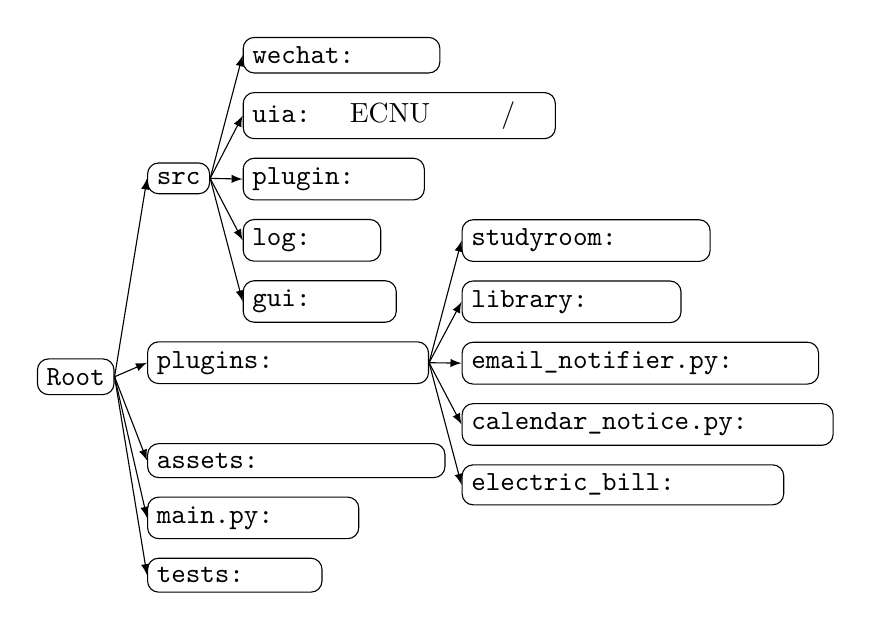
\begin{tikzpicture}
        % 绘制项目结构的树状图
        \node at (0, 0) {
            \begin{forest}
                for tree={
                    grow=east,
                    draw,
                    edge={-latex},
                    rounded corners,
                    node options={align=center, font=\ttfamily},
                    anchor=west,
                    parent anchor=east,
                    child anchor=west,
                    delay={where content={}{shape=coordinate}{}} % 避免错误节点
                }
                % @formatter:off
                [Root
                    [tests: \textnormal{项目早期测试集}]
                    [main.py: \textnormal{软件启动入口文件}]
                    [assets: \textnormal{静态资源目录,包含各开发参考文件及图标等。}]
                    [plugins: \textnormal{各个插件具体实现,可单独删除和添加}
                        [electric\_bill: \textnormal{电费查询及充值提醒插件}]
                        [calendar\_notice.py: \textnormal{课前邮件提醒插件}]
                        [email\_notifier.py: \textnormal{课前邮件提醒插件}]
                        [library: \textnormal{图书馆自动预约插件}]
                        [studyroom: \textnormal{研修间自动预约插件}]
                    ]
                    [src
                        [gui: \textnormal{实现图形用户界面}]
                        [log: \textnormal{实现日志输出}]
                        [plugin: \textnormal{实现插件架构}]
                        [uia: \textnormal{实现 ECNU 统一身份认证辅助/自动登录}]
                        [wechat: \textnormal{实现微信自动控制}]
                    ]
                ]
                % @formatter:on
            \end{forest}
        };
    \end{tikzpicture}
\end{center}

\newpage{} % 第三页结束

\section{项目模块详述}

\subsection{插件登录 ECNU 及辅助登录}

    插件许多功能需要调用 ECNU 提供的各种接口。
    接口的调用依赖于 ECNU 各个系统的登录缓存(在项目内部保存为 \verb`LoginCache`)。
    为了获取有效的登录缓存简化登录操作,
    插件登录使用了 WebDriver 控制浏览器实现自动化或半自动化的辅助登录流程。

    \begin{mdframed}
    本部分代码位于 \texttt{src/uia/login.py} 文件中,核心函数 \texttt{get\_login\_cache} 已提供了完整的注释信息。
    \end{mdframed}

    在插件登录时,会出现浏览器 ECNU 统一身份认证的界面,登录有两种方式。
    \begin{itemize}
        \item 方法一:填写图\ \ref{fig:uia-login-form} 中的表单实现登录。
        \item 方法二:扫描图\ \ref{fig:uia-login-qrcode} 中的二维码实现登录。
    \end{itemize}

    \begin{table}[H]
        \centering
        \begin{tabular}{cc}
            \begin{minipage}[H]{0.372\textwidth}
                \centering
                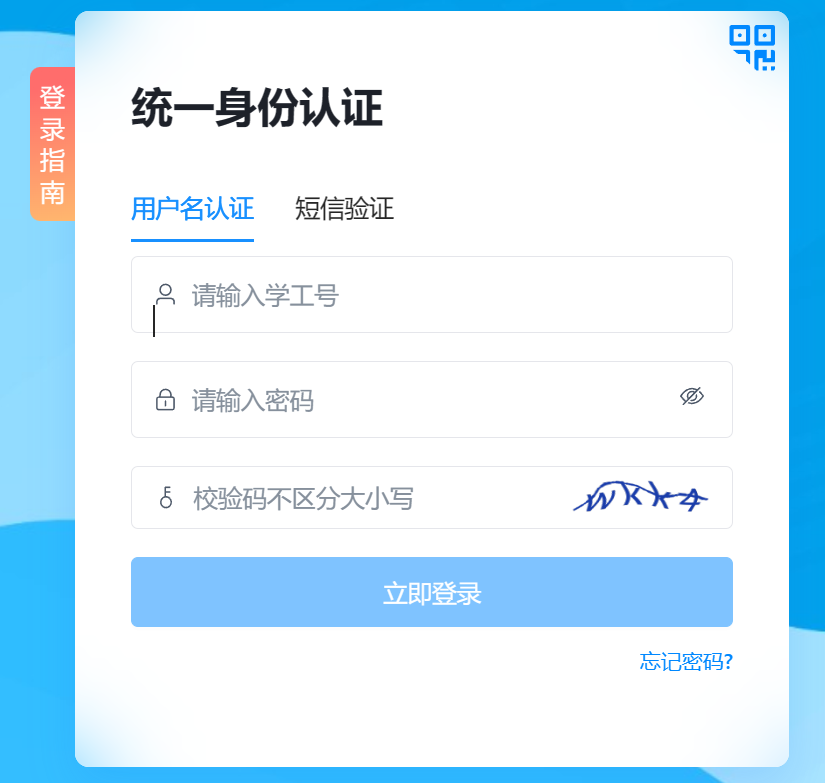
\includegraphics[width=0.8\textwidth]{img/uia_login_form}
                \captionof{figure}{ECNU UIA 登录界面(表单)}
                \label{fig:uia-login-form}
            \end{minipage} &
            \begin{minipage}[H]{0.4\textwidth}
                \centering
                
\includegraphics[width=0.8\textwidth]{img/uia_login_qrcode}
                \captionof{figure}{ECNU UIA 登录界面(二维码)}
                \label{fig:uia-login-qrcode}
            \end{minipage}
        \end{tabular}
    \end{table}

    \begin{rmr}[切换表单登录和二维码登录]
        \quad 表单登录:
        可以在项目根目录创建文件 \verb`login_info.toml`
        然后填写如下内容(替换尖括号以内的部分)。
        插件登录时会读取此文件中的学号密码,自动填写图\ \ref{fig:uia-login-form} 中的表单,实现全自动辅助登录。
        % @formatter:off
        \begin{verbatim}
stu_number = "<填写学号>"
password = "<填写数据库密码>" \end{verbatim}
        % @formatter:on

        \quad 二维码登录:
        删除 \verb`login_info.toml` 文件,
        此时插件辅助登录时会截取二维码图片并发送至邮箱提醒。
        可以使用微信扫描二维码或用微信打开邮件中的连接实现半自动登录。
    \end{rmr}

    \subsubsection{辅助登录大致实现}

    当此软件执行辅助登录的时候:
    
    \begin{description}
        \item[二维码登录]
        进入 ECNU 统一身份认证(下面简称 UIA)界面之后,辅助登录默认使用二维码登录而不是表单登录。
        二维码登录时,脚本截取 UIA 二维码登录图片然后发送到目标邮箱,通过用户微信扫描二维码或者微信打开邮箱中的连接来实现登录。
        \item[表单登录]
        如果创建了 \verb`login_info.toml` 文件(步骤见上述提示),那么脚本会读取其中的学号和密码并自动填写到 UIA 表单中。
        表单中的验证码通过开源库 \href{https://github.com/sml2h3/ddddocr}{DDDDocr} 来识别,成功识别四位验证码之后模拟点击登录按钮来登录。
        如果验证码识别失败则刷新重试。
    \end{description}
    
    成功登录 UIA 之后,各个插件通过自己实现的缓存抓取函数(\textit{Cache Grabber})在各个 ECNU 系统中获得所需要的登录缓存。
    最终,登录缓存通过插件加载器(\textit{Plugin Loader})分发给各个插件。

\newpage{} % 第四页结束

\subsubsection{无状态登录原理}

我们获取的 \texttt{LoginCache} 置于项目根目录中的文件 \texttt{login-cache.pickle} 中,
其中最重要的字段为 \textbf{Bearer} 字段以及 \textbf{cookie} 字段,这是在 \textbf{OAuth 2.0} 框架下在 HTTP 请求头中的认证类型,
携带访问令牌通过 \textbf{Bearer Token} 来实现无状态的认证。

\begin{figure}[H]
    \centering
    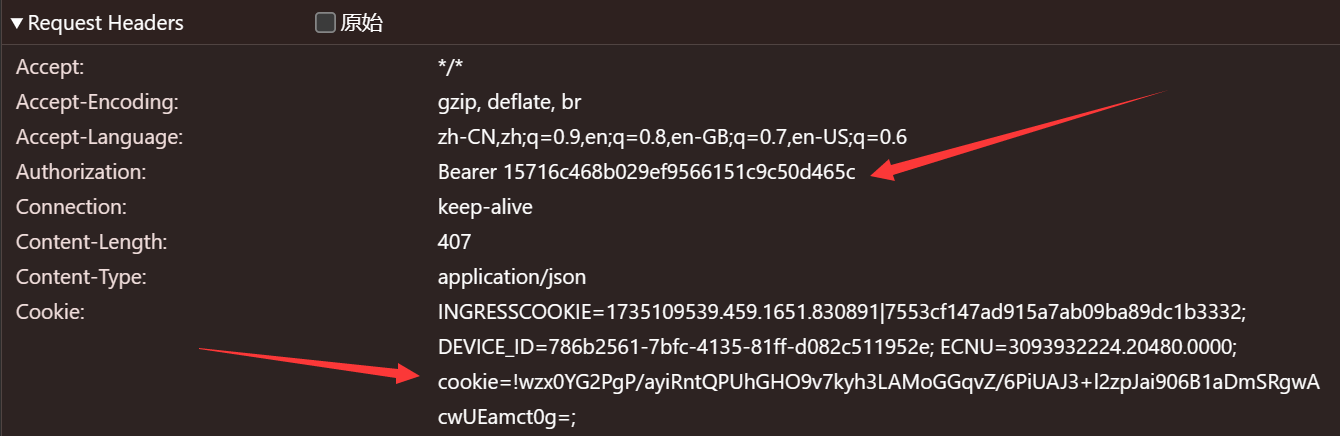
\includegraphics[width=0.66\textwidth]{img/main_cache.png}
    \caption{Main Cookie 及鉴权 Token}
    \label{fig:main_cache}
\end{figure}

正因该 Bearer 字段存在一次获取后便保持一定时长活性的特性,我们才能实现登录缓存的保存机制,为后续分发各缓存至插件提供逻辑闭环(见章节\ \ref{subsec:plugin_loader})。

有时 OCR 的结果不是四位有效的验证码,所以我们添加了一行代码增大了准确性:

\begin{lstlisting}[language=Python]
    if len(captcha) != 4:
        driver.refresh()
\end{lstlisting}

尝试使用后,它有将近 $\frac{2}{3}$ 识别的准确率。此后,便可以实现自动化登录,解放双手了。
较为幸运的是,华师并未设置验证码多次登录失败后禁止登录的逻辑,所以成功率较低的情况下也可以照常使用。

\subsection{插件框架模块}

为了合理地分离代码中的各个逻辑部分,项目构建了插件框架,将不同的功能划分到一个个插件中。插件框架实现了单
独开启和关闭每个插件的功能,让使用者可以根据需要选择希望使用的功能。

\subsubsection{插件加载器(PluginLoader)}\label{subsec:plugin_loader}

项目启动时,PluginLoader 依次导入位于项目根目录下的 \verb`plugins` 文件夹中的插件。
然后从文件中读取各个插件配置,并传递给插件。
插件配置读取完毕之后,PluginLoader 加载各个插件。
被加载的插件可以从其他插件中接收消息和按照特定周期执行(见自然段 \ref{para:routine})。

插件的加载和运行通过 PluginLoader 驱动。它可调用 \verb`get_login_cache()`,
实现各缓存的分发,供相应的插件调用。

\begin{table}[H]
    \centering
    \begin{tabular}{@{}m{0.5\textwidth}@{}m{0.45\textwidth}@{}}
        % 左侧 TikZ 图
        \centering
        \resizebox{0.35\textwidth}{!}{
        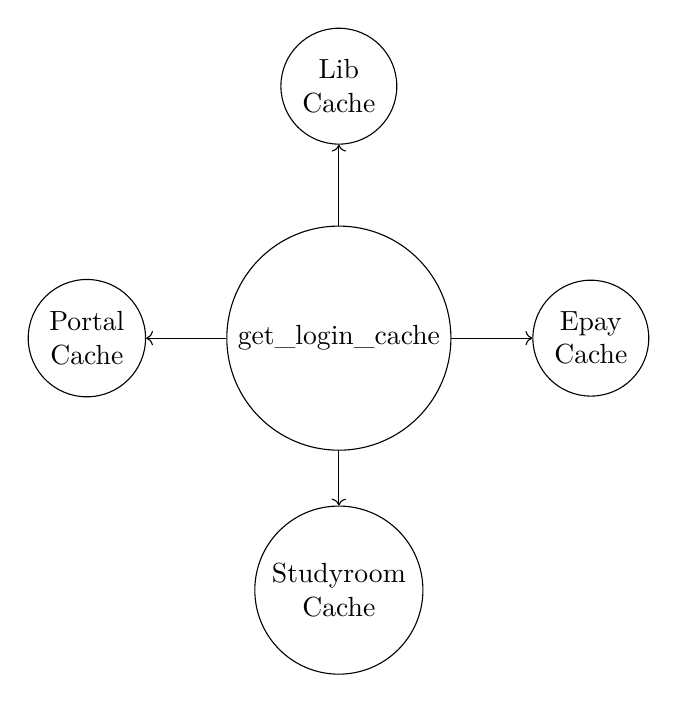
\begin{tikzpicture}[
            node distance=3.2cm,
            every node/.style={draw, circle, minimum size=1.2cm, align=center},
            every edge/.style={draw, thick, -{Latex[length=2mm, width=1mm]}}
            node options={align=center, font=\ttfamily},
        ]
        \node[draw] (center) {get\_login\_cache};
        
        \node[above of=center] (top) {Lib \\ Cache};
        \node[below of=center] (bottom) {Studyroom \\ Cache};
        \node[left of=center] (left) {Portal \\ Cache};
        \node[right of=center] (right) {Epay \\ Cache};
        
        \draw[->] (center) -- (top);
        \draw[->] (center) -- (bottom);
        \draw[->] (center) -- (left);
        \draw[->] (center) -- (right);
        \end{tikzpicture}
        }

        & % 右侧内容介绍
        \raggedright
        \textbf{PluginLoader 具有缓存分发功能}:
        \begin{itemize}
            \item \textbf{Lib Cache}:用于图书馆管理系统。
            \item \textbf{Studyroom Cache}:用于研修间自动预约系统。
            \item \textbf{Portal Cache}:用于公共数据库页面的缓存,目前仅用于课表的获取。
            \item \textbf{Epay Cache}:用于华东师范大学校园卡管理页面的自动查询电费功能。
            \item \textbf{More Cache...}:适配的框架可以获取其余 ECNU 页面的 Cache 以供开发者使用。
        \end{itemize}
    \end{tabular}
    \caption{PluginLoader 的缓存分发与功能说明}
    \label{tab:pluginloader_cache}
\end{table}

\newpage{} % 第五页结束

\subsubsection{插件事件方法}

成功注册后,插件的各种事件方法会被触发,主要的事件方法为:

\paragraph{插件加载和停止(Load 与 Unload)事件}

当插件被加载和停止时触发,插件的加载和停止在插件被导入之后,可能会被使用者多次触发。
用于标记当前插件是否正在运行,方便插件释放资源。代码示例如下:

\begin{lstlisting}[language=python, title = 插件加载和停止示例]
    @register_plugin(
        name="demo_plugin"
    )
    class DemoPlugin(Plugin):
        def on_load(self, ctx: PluginContext):
            pass
        def on_unload(self, ctx: PluginContext):
            pass
\end{lstlisting}

\paragraph{插件周期事件(Routine)}\label{para:routine}
插件在注册的时候可以提供一个回调周期,插件会在指定的回调周期得到回调。示例如下:

\begin{lstlisting}[language=python, title= 周期事件示例]
    @register_plugin(
        name="demo_plugin",
        routine=Routine.MINUTELY
    )
    class DemoPlugin(Plugin):
        def on_routine(self, ctx: PluginContext):
            pass # 周期性得到回调
\end{lstlisting}

\begin{note}
\noindent \textbf{PluginLoader} 根据预定义的频率(Secondly、Minutely、Hourly、Daily、Weekly),调用每个插件的 \texttt{on\_routine} 方法。插件会根据任务频率接收并处理任务,完成对应的功能逻辑。

\vspace{0.3cm}

\noindent 箭头上的 Routine 统一表示调度逻辑,具体任务频率的细节由配置文件决定。例如:
\end{note}

\vspace{0.27cm}

\begin{center}
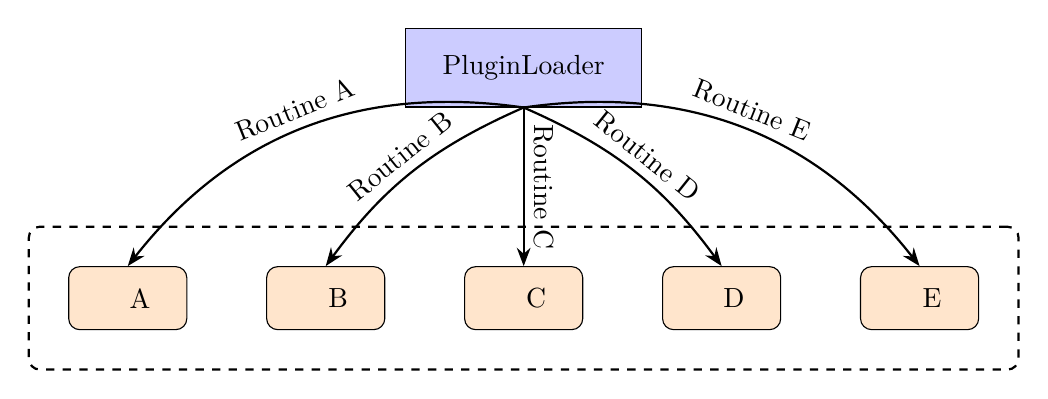
\begin{tikzpicture}[
    plugin/.style={
        rectangle, 
        draw, 
        rounded corners, 
        fill=orange!20, 
        minimum width=1.5cm, 
        minimum height=0.8cm, 
        align=center
    },
    loader/.style={
        rectangle, 
        draw, 
        fill=blue!20, 
        minimum width=3cm, 
        minimum height=1cm, 
        align=center
    },
    dashedbox/.style={
        draw, 
        dashed, 
        thick, 
        rounded corners, 
        inner sep=0.5cm
    },
    arrow/.style={
        ->, 
        thick, 
        >=Stealth
    }
]
    % 定义插件节点,水平排列
    \node (A) [plugin] {插件 A};
    \node (B) [plugin, right=of A] {插件 B};
    \node (C) [plugin, right=of B] {插件 C};
    \node (D) [plugin, right=of C] {插件 D};
    \node (E) [plugin, right=of D] {插件 E};
    
    % 使用 fit 库创建包裹插件的虚线框
    \node [dashedbox, fit=(A) (E)] (dashedbox) {};

    % 将 PluginLoader 放置在虚线框正上方并居中
    \node (loader) [loader, above=1.5cm of dashedbox] {PluginLoader};
        
    % Draw curved arrows from PluginLoader to each plugin
    \draw[arrow, bend right=30] (loader.south) to node[midway, sloped, above] {Routine A} (A.north);
    \draw[arrow, bend right=15] (loader.south) to node[midway, sloped, above] {Routine B} (B.north);
    \draw[arrow] (loader.south) to node [midway, sloped, above] {Routine C} (C.north); % Straight arrow for the middle plugin
    \draw[arrow, bend left=15] (loader.south) to node [midway, sloped, above] {Routine D} (D.north);
    \draw[arrow, bend left=30] (loader.south) to node [midway, sloped, above] {Routine E} (E.north);

\end{tikzpicture}
\end{center}

\subsubsection{插件配置(PluginConfig)}

\begin{mdframed}
    此部分代码如 \verb`root/src/plugin/config.py` 所示。
\end{mdframed}

插件在插件注册时提供需要的配置,在 PluginLoader 从文件中读取插件配置的时候,获得配置的值。

\vspace{0.5cm}

插件配置会集中保存在 \verb`plugin_config.toml` 中,GUI
会为每个插件配置自动生成交互式修改组件,见\ \ref{subsubsec:gui-plugin-config}。
使用者可以通过修改文件或者通过 GUI 修改插件配置。示例如下:

\newpage{}

\begin{lstlisting}[language=python, title = 插件配置示例]
    @register_plugin(
        name="demo_plugin",
        configuration=PluginConfig()
        .add(TextItem(name="first_name", default_value="Tom", description="Your first name"))
    )
    class DemoPlugin(Plugin):
        def on_config_load(self, ctx: PluginContext, cfg: PluginConfig):
            first_name = cfg.get_itme("first_name").current_value
\end{lstlisting}

\begin{note}
    ItemType 中我们定义了许多不同的配置项类型,例如 TextItem、NumberItem、DateItem、PASSWORD 等。
    通过不同类型的定义,可以接受不同的输入,防止用户输入的内容不符合要求,而像 PASSWORD 的定义处理,可以在插件配置界面不明文展示密钥信息,充分保障了信息的安全性。
\end{note}

\begin{figure}[H]
    \centering
    \resizebox{0.8\textwidth}{!}{
        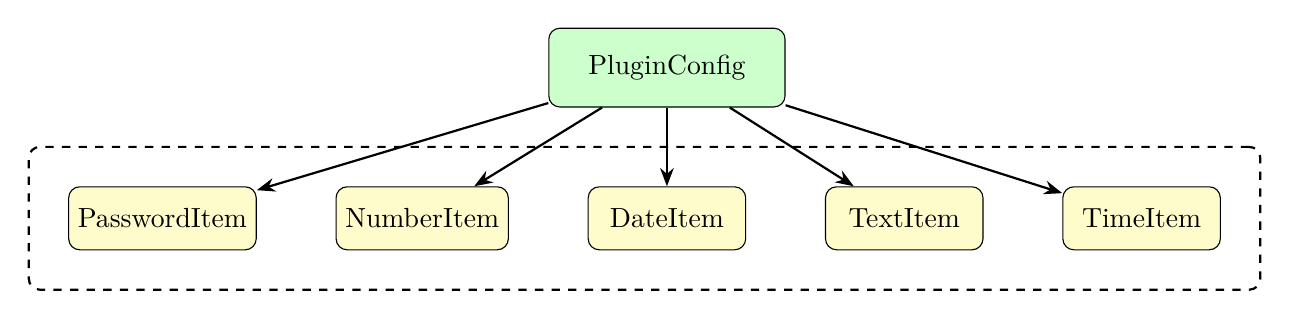
\begin{tikzpicture}[
            pluginconfig/.style={ rectangle, draw, rounded corners, fill=green!20, minimum width=3cm, minimum height=1cm, align=center },
            configitem/.style={ rectangle, draw, rounded corners, fill=yellow!20, minimum width=2cm, minimum height=0.8cm, align=center },
            dashedbox/.style={ draw, dashed, thick, rounded corners, inner sep=0.5cm },
            arrow/.style={ ->, thick, >=Stealth }
        ]
            % Main node
            \node (pluginconfig) [pluginconfig] {PluginConfig};

            % Item nodes
            \node (dateitem) [configitem, below=of pluginconfig] {DateItem};
            \node (textitem) [configitem, right=of dateitem] {TextItem};
            \node (numberitem) [configitem, left =of dateitem] {NumberItem};
            \node (timeitem) [configitem, right=of textitem] {TimeItem};
            \node (passworditem) [configitem, left=of numberitem] {PasswordItem};

            % Dashed box (optional grouping, remove if unnecessary)
            \node [dashedbox, fit= (dateitem) (textitem) (numberitem) (timeitem) (passworditem)] (dashedbox) {};

            % Arrows
            \draw[arrow] (pluginconfig) -- (textitem);
            \draw[arrow] (pluginconfig) -- (numberitem);
            \draw[arrow] (pluginconfig) -- (dateitem);
            \draw[arrow] (pluginconfig) -- (timeitem);
            \draw[arrow] (pluginconfig) -- (passworditem);

        \end{tikzpicture}
    }
    \caption{PluginConfig 和所有 ConfigItem 的关系示意图}
\end{figure}

\subsubsection{插件缓存(PluginCache)}

插件内部生成的数据可以得到统一的持久化保存。插件只需对 PluginCache进行修改,数据会在插件停止时保存,在
插件加载时再次读取。

\begin{lstlisting}[language=python, title=插件缓存示例]
    @register_plugin(
        name="demo_plugin"
    )
    class DemoPlugin(Plugin):
        def on_load(self, ctx: PluginContext):
            ctx.get_logger().info(ctx.get_cache().get("time"))
        def on_routine(self, ctx: PluginContext):
            ctx.get_cache().set("time", time.time())
\end{lstlisting}

\subsubsection{插件上下文(PluginContext)}

\begin{mdframed}
    此部分代码见 \texttt{root/src/plugin/context.py}
\end{mdframed}

\begin{note}
为了保证项目的整洁和规范性,插件创建文件和记录日志等操作使用 PluginContext 进行上下文处理。

每个插件均拥有一个上下文环境,使插件能够与框架进行交互和访问必要的资源。
\end{note}

\begin{figure}[H]
    \centering
    \resizebox{0.95\textwidth}{!}{
    \begin{minipage}[H]{0.4\textwidth}
        \centering
        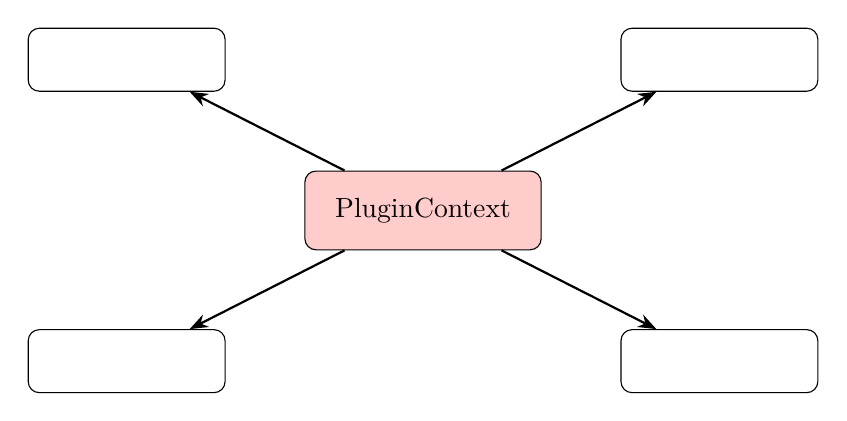
\begin{tikzpicture}[
            context/.style={
                rectangle, 
                draw, 
                rounded corners, 
                fill=red!20, 
                minimum width=3cm, 
                minimum height=1cm, 
                align=center
            },
            feature/.style={
                rectangle, 
                draw, 
                rounded corners, 
                fill=white!80, 
                minimum width=2.5cm, 
                minimum height=0.8cm, 
                align=center
            },
            arrow/.style={
                ->, 
                thick, 
                >=Stealth
            }
        ]
        
        % PluginContext Node
        \node (context) [context] {PluginContext};
        
        % Features of PluginContext
        \node (logger) [feature, above left=of context] {日志记录器};
        \node (cache) [feature, above right=of context] {读写登录缓存};
        \node (message) [feature, below left=of context] {消息传递};
        \node (actions) [feature, below right=of context] {用户操作绑定};
        
        % Arrows from PluginContext to Features
        \draw[arrow] (context) -- (logger);
        \draw[arrow] (context) -- (cache);
        \draw[arrow] (context) -- (message);
        \draw[arrow] (context) -- (actions);
        
        \end{tikzpicture}
    \end{minipage}
    \hspace{2.5cm}
    \begin{minipage}[H]{0.6\textwidth}
        \textbf{PluginContext 的功能组成}:
        \begin{itemize}
            \item \textbf{日志记录}:
            插件专属的日志记录(信息、警告、错误等)。
            \item \textbf{读写登录缓存}:
            插件可以通过 \texttt{ctx.get\_cache()} 访问自己的持久化缓存,用于存储跨会话的数据。
            缓存支持数据的读取和写入,确保插件状态的持久性。
            \item \textbf{消息传递}:
            向其他插件发送消息
            \item \textbf{用户操作绑定}:
            可创建可交互按钮(Bind Action),相应的回调函数执行对应操作。
        \end{itemize}
    \end{minipage}
    }
\end{figure}

\subsubsection{插件消息传递(Message)}

插件通过 PluginContext 可以向其他插件发送消息。发送示例如下:

\begin{lstlisting}[language=python, title = 发送消息示例]
    @register_plugin(
        name="send_demo_plugin"
    )
    class DemoPlugin(Plugin):
        def on_routine(self, ctx: PluginContext):
            ctx.send_message("recv_demo_plugin", "Hello World")
    
    @register_plugin(
        name="recv_demo_plugin"
    )
    class RecvPlugin(Plugin):
        def on_recv(self, ctx: PluginContext, from_plugin: str, obj: Any):
            ctx.get_logger().info((from_plugin, obj))
\end{lstlisting}

\subsection{课前提醒模块}

\subsubsection{模块设计与配置}

\begin{mdframed}
    本模块位于 \texttt{plugins/studyroom/calendar\_notice\_plugin.py}
\end{mdframed}

本插件在设计上,主要用于与其他插件通信。
查询最近的课表并发送邮件提醒用户只是最简单的功能。

\begin{note}
通过插件通信,可以通知其他插件(如研修间预约与图书馆预约模块),若一定时间内没有课程,其他模块便可以开始调用相应的预约接口。
我们的设计为:查询当前时刻至次日该时刻用户的课程安排,如果有课程,上课前的一定时段发送邮件提醒用户去上课。
可以通过插件配置来配置上课前多久提醒用户。
\end{note}

\begin{figure}[H]
    \centering
    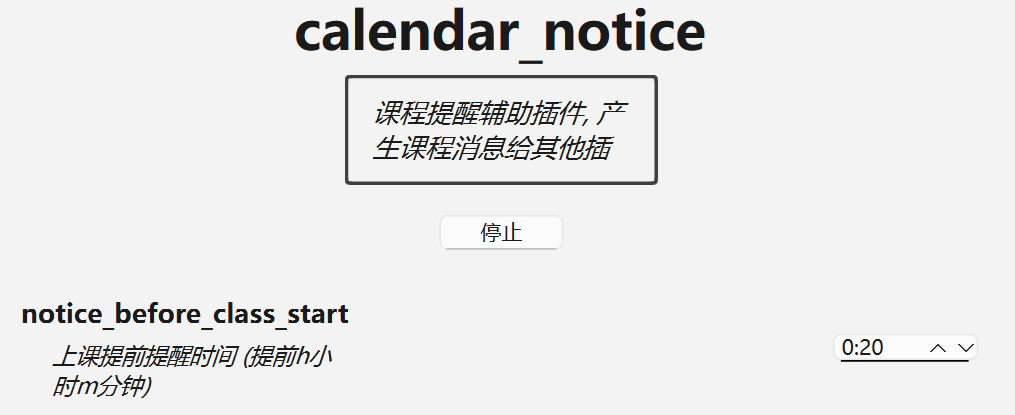
\includegraphics[width=0.6\textwidth]{img/calendar_notice_config.png}
    \caption{课前提醒模块配置}
    \label{fig:calendar_notice_config}
\end{figure}

\newpage{}

\subsubsection{课表获取及数据处理原理}

\begin{table}[H]
    \centering
    \begin{tabular}{cc}
        \begin{minipage}[H]{0.4\textwidth}
            \centering
            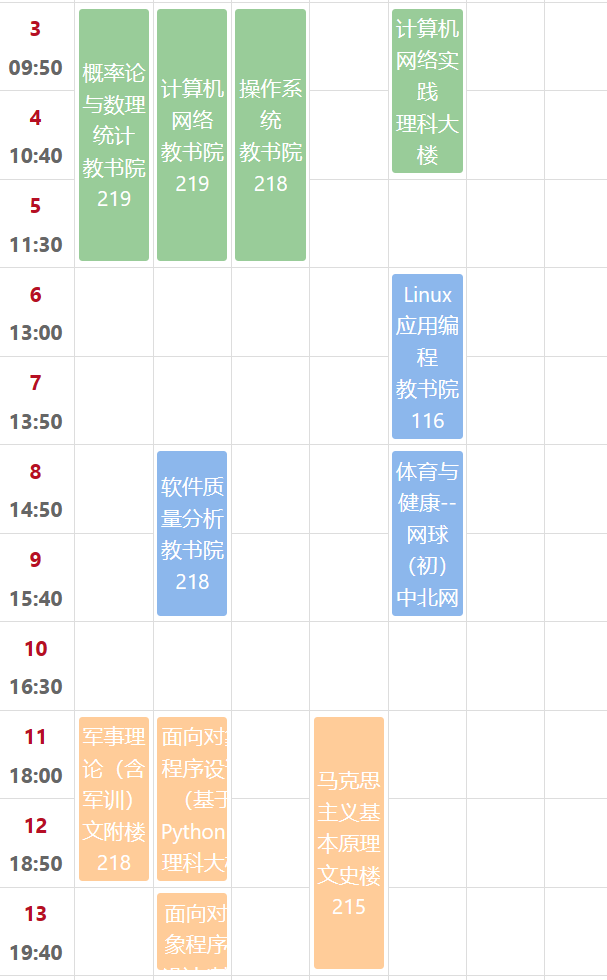
\includegraphics[width=0.5\textwidth]{img/calendar.png}
            \captionof{figure}{ECNU Portal 课表页面}
            \label{fig:login}
        \end{minipage} &
        \begin{minipage}[H]{0.5\textwidth}
            \raggedright
            进入电脑端 Portal 主页面右侧,我们可以看到自己的课表,使用 Selenium-Wire 抓包得知,
            实际上,本课表是存在一个请求 Url 的。
            
            \vspace{0.5cm}
            
            那么我们通过上述获得的 \verb`login_cache`,携带 \textbf{Bearer} 鉴权字段和对应的 \textbf{Cookie},通过 requests 库发起请求,即可实时获取课表。
        \end{minipage}
    \end{tabular}
\end{table}

\begin{figure}[H]
    \centering
    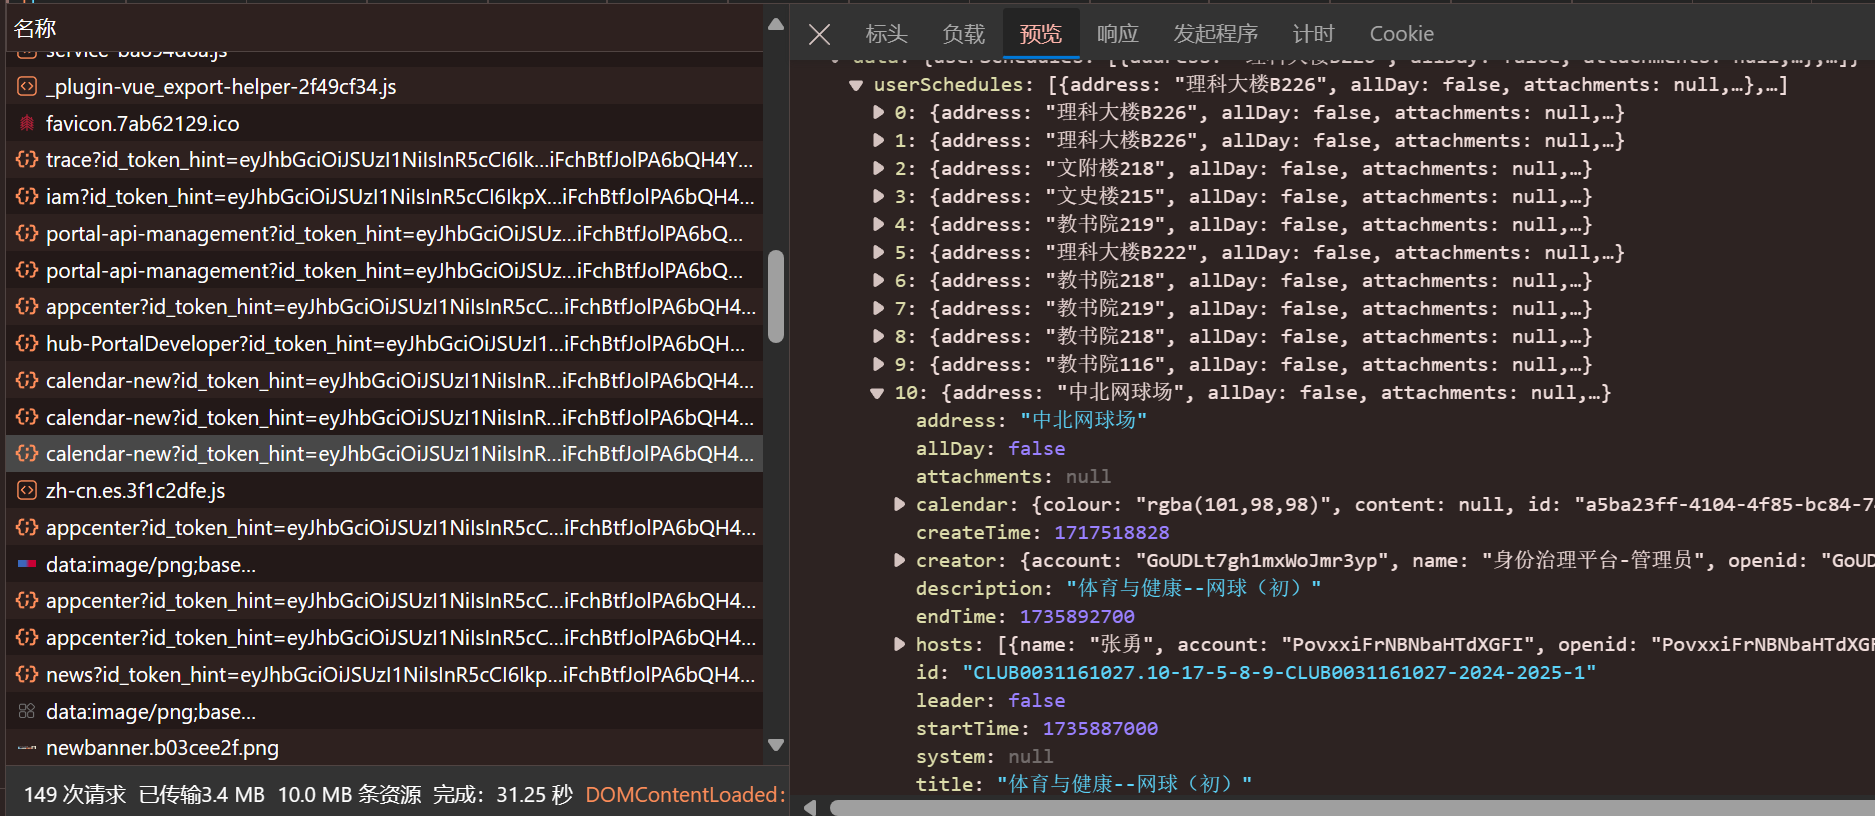
\includegraphics[width=0.7\textwidth]{img/calendar-new-url.png}
    \caption{Portal 课表请求}
    \label{fig:portal_course_table}
\end{figure}

这个 POST 请求采用的是 GraphQL 的查询格式,我们只需要使用 filter 过滤器查询自己所需要的字段即可。

\begin{lstlisting}[language=python]
    USER_SCHEDULES = """
    query ($filter: ScheduleFilter, $userId: String) {
      userSchedules(filter: $filter, userId: $userId) {
        address # 上课地点
        hosts {
          name # 教师名字
        }
        description # 课程信息和描述
        endTime # 结束时间
        startTime # 开始时间
      }
    }
    """
\end{lstlisting}

\begin{itemize}
    \item 获取用户从此刻至第二天此时的课表后,将每一个课程的时间戳转换后与当前的时间进行比较,
    \item 若小于了用户设置的提醒时间,则发送邮件提醒用户。
\end{itemize}

\newpage{}

\subsection{研修间预约模块}

\subsubsection{代码框架及配置}

此部分代码位于 \texttt{src/studyroom/} 中。

\begin{figure}[H]
    \centering
    \resizebox{\textwidth}{!}{
    \begin{minipage}[H]{0.5\textwidth}
        \centering
        \begin{forest}
            for tree={
                grow=east,
                draw,
                edge={-latex},
                rounded corners,
                node options={align=center},
                anchor=west,
                parent anchor=east,
                child anchor=west,
                delay={where content={}{shape=coordinate}{}} % 避免错误节点
            }
            [root
                [src
                    [studyroom
                        [\_\_init\_\_.py]
                        [available.py]
                        [query.py]
                        [req.py]
                        [studyroom\_plugin.py]
                        [subscribe.py]
                    ]
                ]
            ]
        \end{forest}
    \end{minipage}

    \hspace{0.8cm}

    \begin{minipage}[H]{0.45\textwidth}
        \raggedright
        \textbf{模块说明:}\\
        \vspace{0.2cm}
        \textbf{Query (\texttt{query.py})}\\
        该模块仅实现对 \texttt{url} 的简单请求,不作任何数据处理。它通过相应的 API 获取研修室的可用性和详细信息。\\
        \vspace{0.4cm}

        \textbf{Available (\texttt{available.py})}\\
        \texttt{available.py} 模块负责处理房间可用性数据。它分析当前和已预订的时间段,确定研修室可预约的时间段。\\
        \vspace{0.4cm}

        \textbf{Subscribe (\texttt{subscribe.py})}\\
        \texttt{subscribe.py} 模块管理预约流程。它包括进行预约、检查预约状态以及在特定条件下自动取消预约的功能。
    \end{minipage}
    }
    \caption{研修间的目录结构及模块说明}
    \label{fig:directory_structure}
\end{figure}

\rule{0.87\textwidth}{0.4pt} % 添加一条跨越页面宽度的横线,厚度为 0.4pt

配置好后,软件会自动计算当前时间和下次上课时间的间隔,并判断是否符合预约条件。

\begin{figure}[H]
    \centering
    \begin{tabular}{@{}m{0.55\textwidth}@{}m{0.4\textwidth}@{}}
        % 左侧文字描述
        \begin{minipage}[H]{\linewidth}
            \textbf{研修间配置说明}:
            \begin{itemize}[label=--]
                \item \textbf{min\_reserve\_time}:最短预约时长。最小值为 \texttt{1:00}。
                \item \textbf{max\_reserve\_time}:最长预约时长。最大值为 \texttt{4:00}。
                \item \textbf{auto\_cancel}:
                \begin{itemize}
                    \item \texttt{1} (\textbf{True}):自动取消即将过期的预约。
                    \item \texttt{0} (\textbf{False}):不自动取消。
                \end{itemize}
                \item \textbf{reserve\_place}:
                \begin{itemize}
                    \item 普陀校区木门研修室、玻璃门研修室
                    \item 闵行校区研修室
                \end{itemize}
            \end{itemize}
        \end{minipage}
        &
        \begin{minipage}[H]{\linewidth}
            \centering
            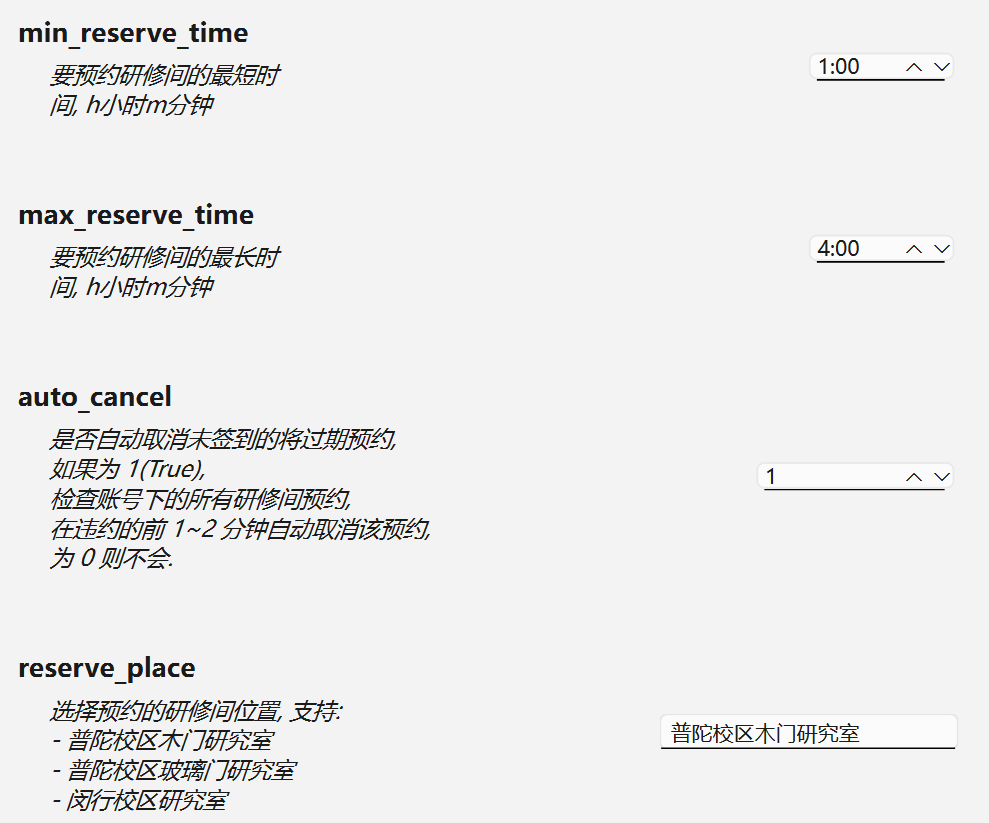
\includegraphics[width=\linewidth]{img/studyroom_config.png}
            \label{fig:studyroom_config}
        \end{minipage}
    \end{tabular}
\end{figure}

\subsubsection{研修间预约实现原理}

华东师范大学研修间预约最少预约时长在 60 分钟以上,最长不能超过 240 分钟。对于单人学生,仅有
普陀校区木门研究室、闵行校区研究室、普陀校区玻璃门研究室可供单人预约使用。

查看研修间的预约情况,我们首先从这一张研修间状态列表中计算出可用时间(AvailableInfos)都有哪些:

\begin{figure}[H]
    \centering
    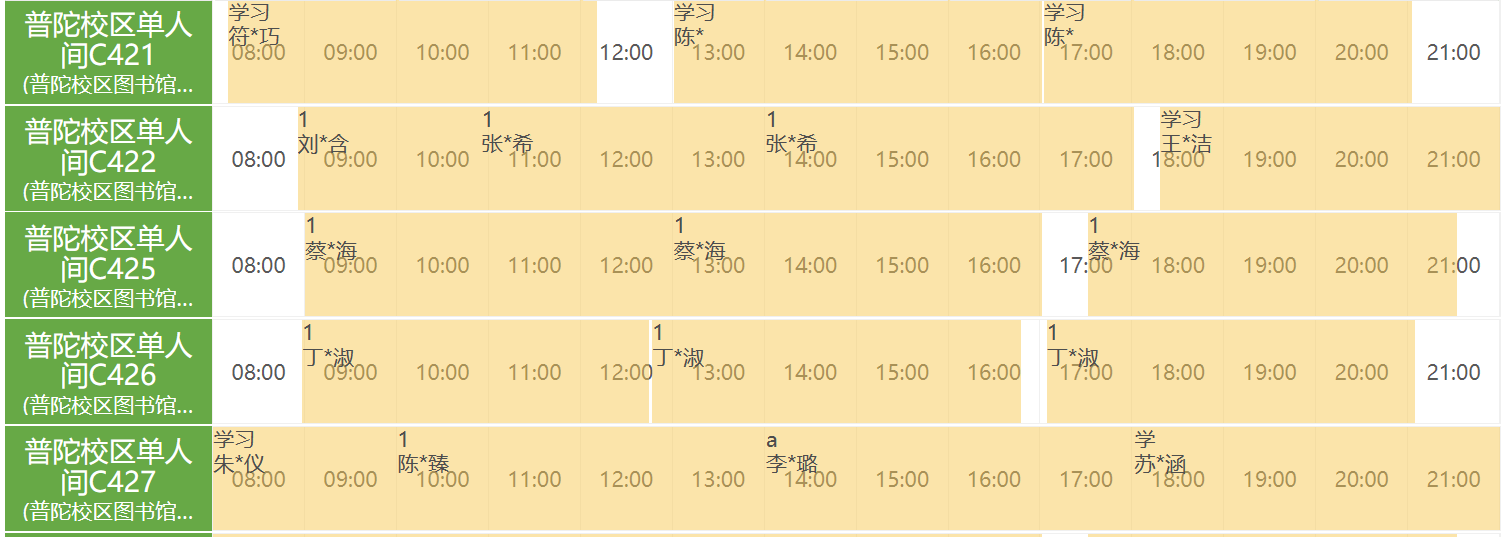
\includegraphics[width=0.62\textwidth]{img/studyroom_state.png}
    \caption{研修间状态示例}
    \label{fig:studyroom_available}
\end{figure}

加载入网页时,该Url会自动调用:\href{https://studyroom.ecnu.edu.cn/ic-web/roomDevice/roomAvailable}{\underline{https://studyroom.ecnu.edu.cn/ic-web/roomDevice/roomAvailable}}
拥有查询当前类别的研修间的功能,其返回的字段如下:

\begin{lstlisting}[language=python]
    {'devId': 3676503,                             # 设备 ID
    'devName': '普陀校区单人间C421',                # 设备名称
    'minResvTime': 60,                             # 最小预约时间
    'openTimes': [{'openEndTime': '22:00',         # 开放结束时间
                   'openLimit': 1,                 # 最少预约人数
                   'openStartTime': '08:00'}],     # 开放开始时间
    'resvInfos': [{'resvBeginTime': '2024-12-26 '  # (People No.1) 的预约信息
                                    '17:01:00',
                   'resvEndTime': '2024-12-26 '
                                  '21:01:00',
                   'resvStatus': 1093}]},
\end{lstlisting}

它只为我们提供了 \texttt{'resvInfos'} 字段,这应该是用于前端供渲染黄色已预定时间段的给用户的,
所以我们需要将它与 \texttt{'openTimes'} 字段结合起来,得到研修室的可用时间段。

\begin{note}
    \begin{itemize}
        \item 将 [openStartTime, currentTime] 区间视为不可用时间段。例如当天 18:55 P.M 前的时间段都无效。
        \item 仅 AvailableTime > minResvTime 时,才将这段区间设置为 AvailableTime, 不考虑未超过最短预约时间的情况。
    \end{itemize}
\end{note}

返回的信息字典中,我们通过程序包含了一个新字段 \texttt{availableInfos},这样就可以提供给用户可用的时间段了。

之后,使用 \texttt{reserve.py} 中的函数 \texttt{\_fetch\_userInfo} 来获取 \texttt{appAccNo},这是识别用户身份的字段,
在发送 \texttt{reserve} 请求时,需要传入该字段作为 Payload 的一部分。最后通过调用 \texttt{reserve\_room} 函数即可完成全自动预约。

\begin{note}
每一次预约都会形成一个唯一的预约编号,称为 \texttt{uuid},我们在进入个人中心时,网页会自动调用查询的接口:

\href{https://studyroom.ecnu.edu.cn/#/ic/userinfo}{\underline{https://studyroom.ecnu.edu.cn/\#/ic/userinfo}}
,所以,我们也可以通过抓包获取 uuid,便可以知道用户当前是否有预约了,这为后续的自动取消预约提供了保障。
\end{note}

研修间预约时,需要提交的表单样式如下,我们不采用浏览器自动操作的形式,而是截取提交时发送的 url 请求:

\begin{figure}[H]
    \centering
    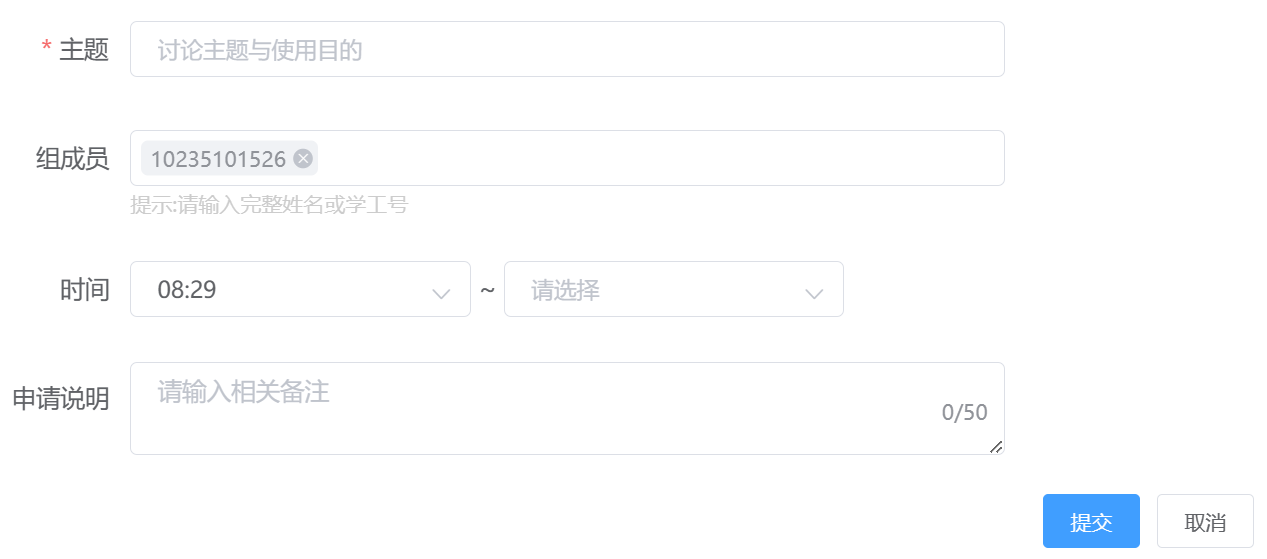
\includegraphics[width=0.5\textwidth]{img/studyroom_submit.png}
    \caption{研修间预约表单}
    \label{fig:studyroom_reserve}
\end{figure}

抓包得到 POST 请求的 Url 如下:\href{https://studyroom.ecnu.edu.cn/ic-web/reserve}{\underline{https://studyroom.ecnu.edu.cn/ic-web/reserve}}

只需传入相关的字段即可:

\begin{figure}[H]
    \centering
    \begin{minipage}[H]{0.45\textwidth} % 左侧放图片
        \centering
        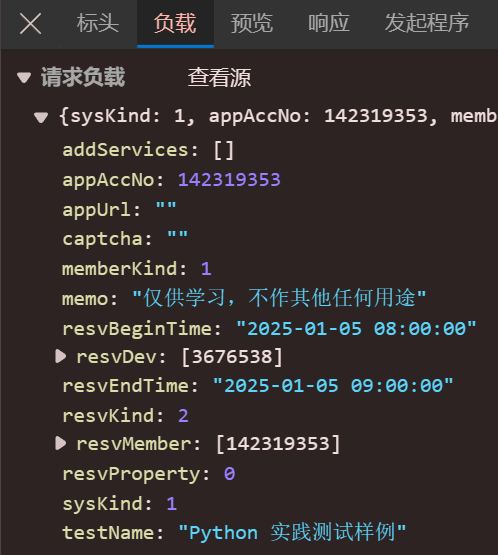
\includegraphics[width=0.75\textwidth]{img/studyroom_request.png}
        \caption{研修间预约请求}
        \label{fig:studyroom_request}
    \end{minipage}
    \hspace{0.05\textwidth} % 图片和代码之间的间距
    \begin{minipage}[H]{0.45\textwidth} % 右侧放代码
        \centering
        \begin{lstlisting}[language=python, caption={预约请求需要传入的字段}]
headers = {
    "Cookie": f"ic-cookie={ic_cookie}", 
} # 从 StudyroomCache 中获取 ic-cookie

# 从 _fetch_userInfo 获取用户 ID
appAccNo = self._fetch_userInfo().get("accNo")

payload = {
    "sysKind": 1,  # 系统类型,默认为 1
    "appAccNo": appAccNo,
    "memberKind": 1,  # 成员类型,默认为 1
    "resvBeginTime": resvBeginTime,
    "resvEndTime": resvEndTime,
    "testName": testName,
    "resvMember": [appAccNo],
    # 默认预约人员列表只有当前用户
    "resvDev": resvDev,
    "memo": memo,
}
        \end{lstlisting}
    \end{minipage}
\end{figure}

\subsection{图书馆预约模块}

\subsubsection{代码框架及分析}

\begin{figure}[H]
    \centering
    \resizebox{\textwidth}{!}{
    \begin{minipage}[H]{0.5\textwidth}
        \centering
        \begin{forest}
            for tree={
                grow=east,
                draw,
                edge={-latex},
                rounded corners,
                node options={align=center},
                anchor=west,
                parent anchor=east,
                child anchor=west,
                delay={where content={}{shape=coordinate}{}} % Avoid empty nodes
            }
            [root
                [plugins
                    [library
                        [\_\_init\_\_.py]
                        [date.py]
                        [encrypt.py]
                        [library\_plugin.py]
                        [query.py]
                        [req.py]
                        [seat.py]
                        [subscribe.py]
                        [tests.py]
                    ]
                ]
            ]
        \end{forest}
    \end{minipage}

    \hspace{0.8cm}

    \begin{minipage}[H]{0.45\textwidth}
        \raggedright
        \textbf{部分模块功能说明:}\\
        \vspace{0.25cm}

        \textbf{Encrypt (\texttt{encrypt.py})}\\
        提供加密与解密功能,使用 AES 加密算法保障数据传输安全,通过填充和密钥生成实现加密。\\
        \vspace{0.25cm}

        \textbf{Seat (\texttt{seat.py})}\\
        提供座位数据对象化表示,实现计算座位间距离、判断空闲状态等功能,并包括寻找最优座位的算法。\\
        \vspace{0.25cm}

        \textbf{Subscribe (\texttt{subscribe.py})}\\
        实现座位预约的核心逻辑,包括预约、查询、取消功能,并通过加密模块保障传输安全。\\
        \vspace{0.25cm}

        \textbf{Library Plugin (\texttt{library\_plugin.py})}\\
        提供座位预约插件,支持快速预约、用户配置偏好和自动取消未签到预约等功能。\\
        \vspace{0.25cm}

        \textbf{Query (\texttt{query.py})}\\
        封装查询接口,包括查询座位空闲情况、具体座位信息、可用时间段等,并支持按条件筛选区域和座位。\\
    \end{minipage}
    }
    \caption{ECNU 图书馆预约模块说明}
    \label{fig:directory_structure}
\end{figure}

\newpage{}

\begin{table}[H]
    \centering
    \begin{tabular}{@{}m{0.55\textwidth}@{}m{0.4\textwidth}@{}}
        % 左侧文字
        \begin{minipage}[H]{\linewidth}
            \textbf{配置说明:}
            \begin{itemize}[label=--]
                \item \textbf{prefer\_study\_duration}:偏好的学习时长
                \item \textbf{auto\_cancel}:是否自动取消未签到的过期预约
                \begin{itemize}
                    \item \texttt{1 (True)}:会在预约到期前 1~2 分钟自动取消
                    \item \texttt{0 (False)}:不会自动取消
                \end{itemize}
                \item \textbf{premise}:预约座位选择的校区
            \end{itemize}
        \end{minipage}
        &
        % 右侧图片
        \begin{minipage}[H]{\linewidth}
            \centering
            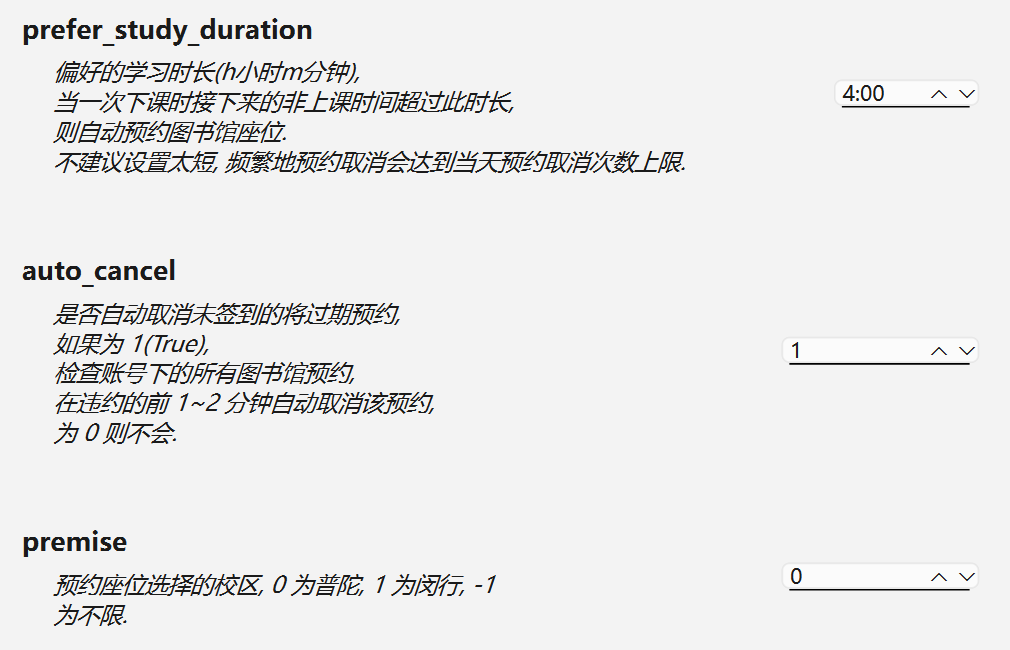
\includegraphics[width=\linewidth]{img/library_plugin_config.png}
            \caption{图书馆预约配置}
            \label{fig:library_config}
        \end{minipage}
    \end{tabular}
\end{table}

\subsubsection{图书馆预约实现原理}

系统使用了Axios的请求拦截器来对特定API请求进行加密。以下是相关的JavaScript代码片段:

% 暂不支持 JavaScript 代码高亮, 用 Python 代码代替
\begin{lstlisting}[language=C, caption=请求拦截与加密代码]
service.interceptors.request.use(function(config) {
    let encryptRequest = ["/api/login/resetpass", "/api/login/login", "/api/login/forget", "/api/Seat/confirm", "/api/Seminar/confirm", "/reserve/index/confirm", "/api/Enter/confirm", "/api/Seat/touch_qr_books", "/api/seat/qrcode", "/api/seat/qrcode_not_card", "/api/Study/StudyOrder", "/api/login/updateUserInfo", "/api/seat/xuzuoconfirm"],
    token = sessionStorage.getItem("token") || "",
    lang = localStorage.getItem("lang") || "zh";
    
    if (token) {
        // 处理已登录状态下的请求
        if (encryptRequest.includes(config.url)) {
            let encryptedData = encrypt("encrypt", config.data);
            config.data = encryptedData;
        }
        // 其他处理逻辑...
    } else {
        // 处理未登录状态下的请求
        if (encryptRequest.includes(config.url)) {
            let encryptedData = encrypt("encrypt", config.data);
            config.data = encryptedData;
        }
        // 其他处理逻辑...
    }
    // 其他配置...
    return config;
});
\end{lstlisting}

\paragraph{请求拦截器解析}

上述代码通过Axios的请求拦截器,对特定API路径的请求数据进行加密处理。主要步骤包括:

\begin{enumerate}
    \item 定义需要加密的API路径数组\texttt{encryptRequest}。
    \item 从\texttt{sessionStorage}和\texttt{localStorage}中获取\texttt{token}和\texttt{lang}。
    \item 判断当前请求的URL是否在需要加密的列表中。
    \item 如果需要加密,则调用\texttt{encrypt}函数对请求数据进行加密。
\end{enumerate}

\paragraph{加密函数分析}

加密操作主要集中在\texttt{encrypt}函数中。以下是该函数的具体实现:

\begin{lstlisting}[language=C, caption=加密函数代码]
    function encrypt(g, y) {
        var k = exchangeDateTime(new Date, 41);
        // `.split("")`: 按照每个字符分割字符串.
        k = `${k}${k.split("").reverse().join("")}`; // AES 密钥.
        // 调试发现 k 可能为 "2024112882114202", 就是当前日期年月日这个字符串和他的倒转相加.
        var j = k;
        var pe = "ZZWBKJ_ZHIHUAWEI"; // AES iv 向量.
        if (g == "encrypt")
            // 加密操作, 见下文.
            return crypto.encrypt(JSON.stringify(y), j, pe);
        ...
    }
    const CryptoJS = cryptoJs.exports
    const crypto = {
        encrypt(g, j, pe) { // 这里的 j 就是密钥, 就是上文 encrypt 中的 k 变量.
            // CryptoJS.enc.Utf8.parse 是 CryptoJS 中的一个方法
            // 用于将普通字符串转换为 CryptoJS 的 WordArray 对象, 不涉及加密操作.
            var j = CryptoJS.enc.Utf8.parse(j);
            var pe = CryptoJS.enc.Utf8.parse(pe);
            var Ce = CryptoJS.AES.encrypt(g, j, { // CryptoJS.AES.encrypt(message, key, options)
                iv: pe,
                mode: CryptoJS.mode.CBC,
                padding: CryptoJS.pad.Pkcs7
            });
            return Ce.toString()
        }
    };
\end{lstlisting}

\subsubsection*{加密过程详解}

\begin{enumerate}
    \item \textbf{密钥生成}:
    \begin{itemize}
        \item 调用\texttt{exchangeDateTime}函数获取当前日期时间,并传入参数41进行处理,生成基础密钥\texttt{k}。
        \item 将\texttt{k}与其倒序字符串拼接,形成最终的AES密钥。
        \item 例如,如果\texttt{k}为\texttt{"2024112882114202"},则最终密钥为\texttt{"20241128821142022024112882114202"}。
    \end{itemize}
    
    \item \textbf{初始化向量(IV)}:
    \begin{itemize}
        \item 固定IV值为\texttt{"ZZWBKJ\_ZHIHUAWEI"}。
    \end{itemize}
    
    \item \textbf{加密操作}:
    \begin{itemize}
        \item 使用\texttt{CryptoJS}库进行AES加密,采用CBC模式和Pkcs7填充。
        \item 将待加密的数据序列化为JSON字符串后进行加密。
        \item 返回加密后的Base64字符串。
    \end{itemize}
\end{enumerate}

\subsubsection*{Python 实现加密过程}

\vspace{0.3cm}

\begin{lstlisting}[language=Python, caption=Python加密复现代码]
    def encrypt(cls, json_data: dict, key: str = None) -> str:
        """
        加密函数,加密数据并返回加密 base64 字符串。

        >>> Encryptor.encrypt({"seat_id": "3361", "segment": "1508173"}, "2024112882114202")
        '6l1+11NSwbo9Rje1/+pnuSqexfDXg/pPDTK0KJEG/uOIZyucecgEo7VO8ggVRom9'
        """
        if key is None:  # 这个默认值
            key = day_str()
            key = key + key[::-1]
        to_encrypt = json.dumps(json_data, separators=(",", ":")).encode("utf-8")
        en = AES.new(
            key=key.encode("utf-8"),
            mode=AES.MODE_CBC,
            iv=AES_IV.encode("utf-8"),
        )
        return base64.b64encode(
            en.encrypt(pkcs7_pad(to_encrypt, AES.block_size))
        ).decode('utf-8')
\end{lstlisting}

\subsection{电费查询模块}

电费查询插件用到了服务端和客户端,两个客户端之间通过 \verb`iv` 与 \verb`key` 进行加密通信,以确保数据安全与隐私性。

\newpage{}

\section{项目主要界面贴图}

整体的 GUI 设计使用 Pyside 6 进行开发,以下是各个页面的贴图及简单介绍。

\subsection{主页}

标题栏显示项目标题和登录状态,左侧是标签页切换按钮,右侧是主页大标题和登录、退出软件两个按钮,见图 \ref{fig:home}

\begin{figure}[H]
    \centering
    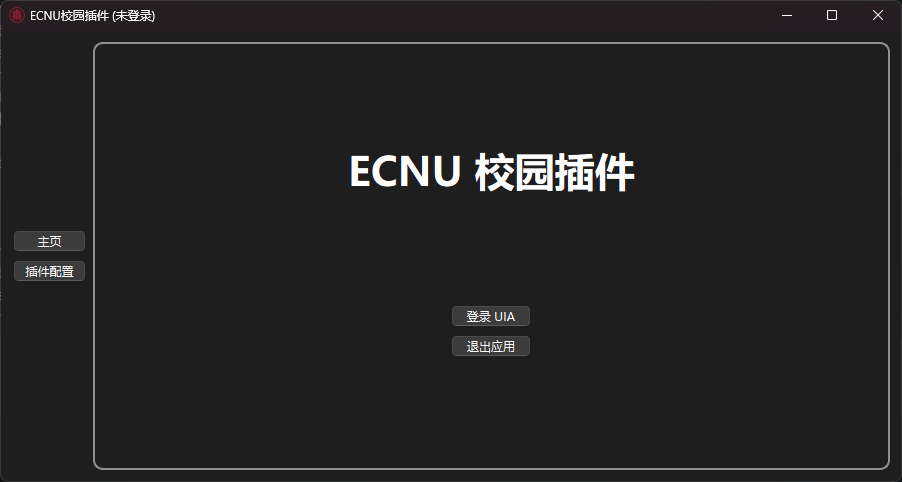
\includegraphics[width=0.6\textwidth]{img/home}
    \caption{主页}
    \label{fig:home}
\end{figure}

\subsection{插件配置页面}\label{subsubsec:gui-plugin-config}

插件配置页面右侧框中左侧的列表是插件选择,鼠标单击即可进入各个插件的配置界面,如图\ref{fig:plugin-config-gui} 中红框所示。

在每个插件的配置界面,会根据插件注册时提供的配置项生成可交互配置界面。

\begin{figure}[H]
    \centering
    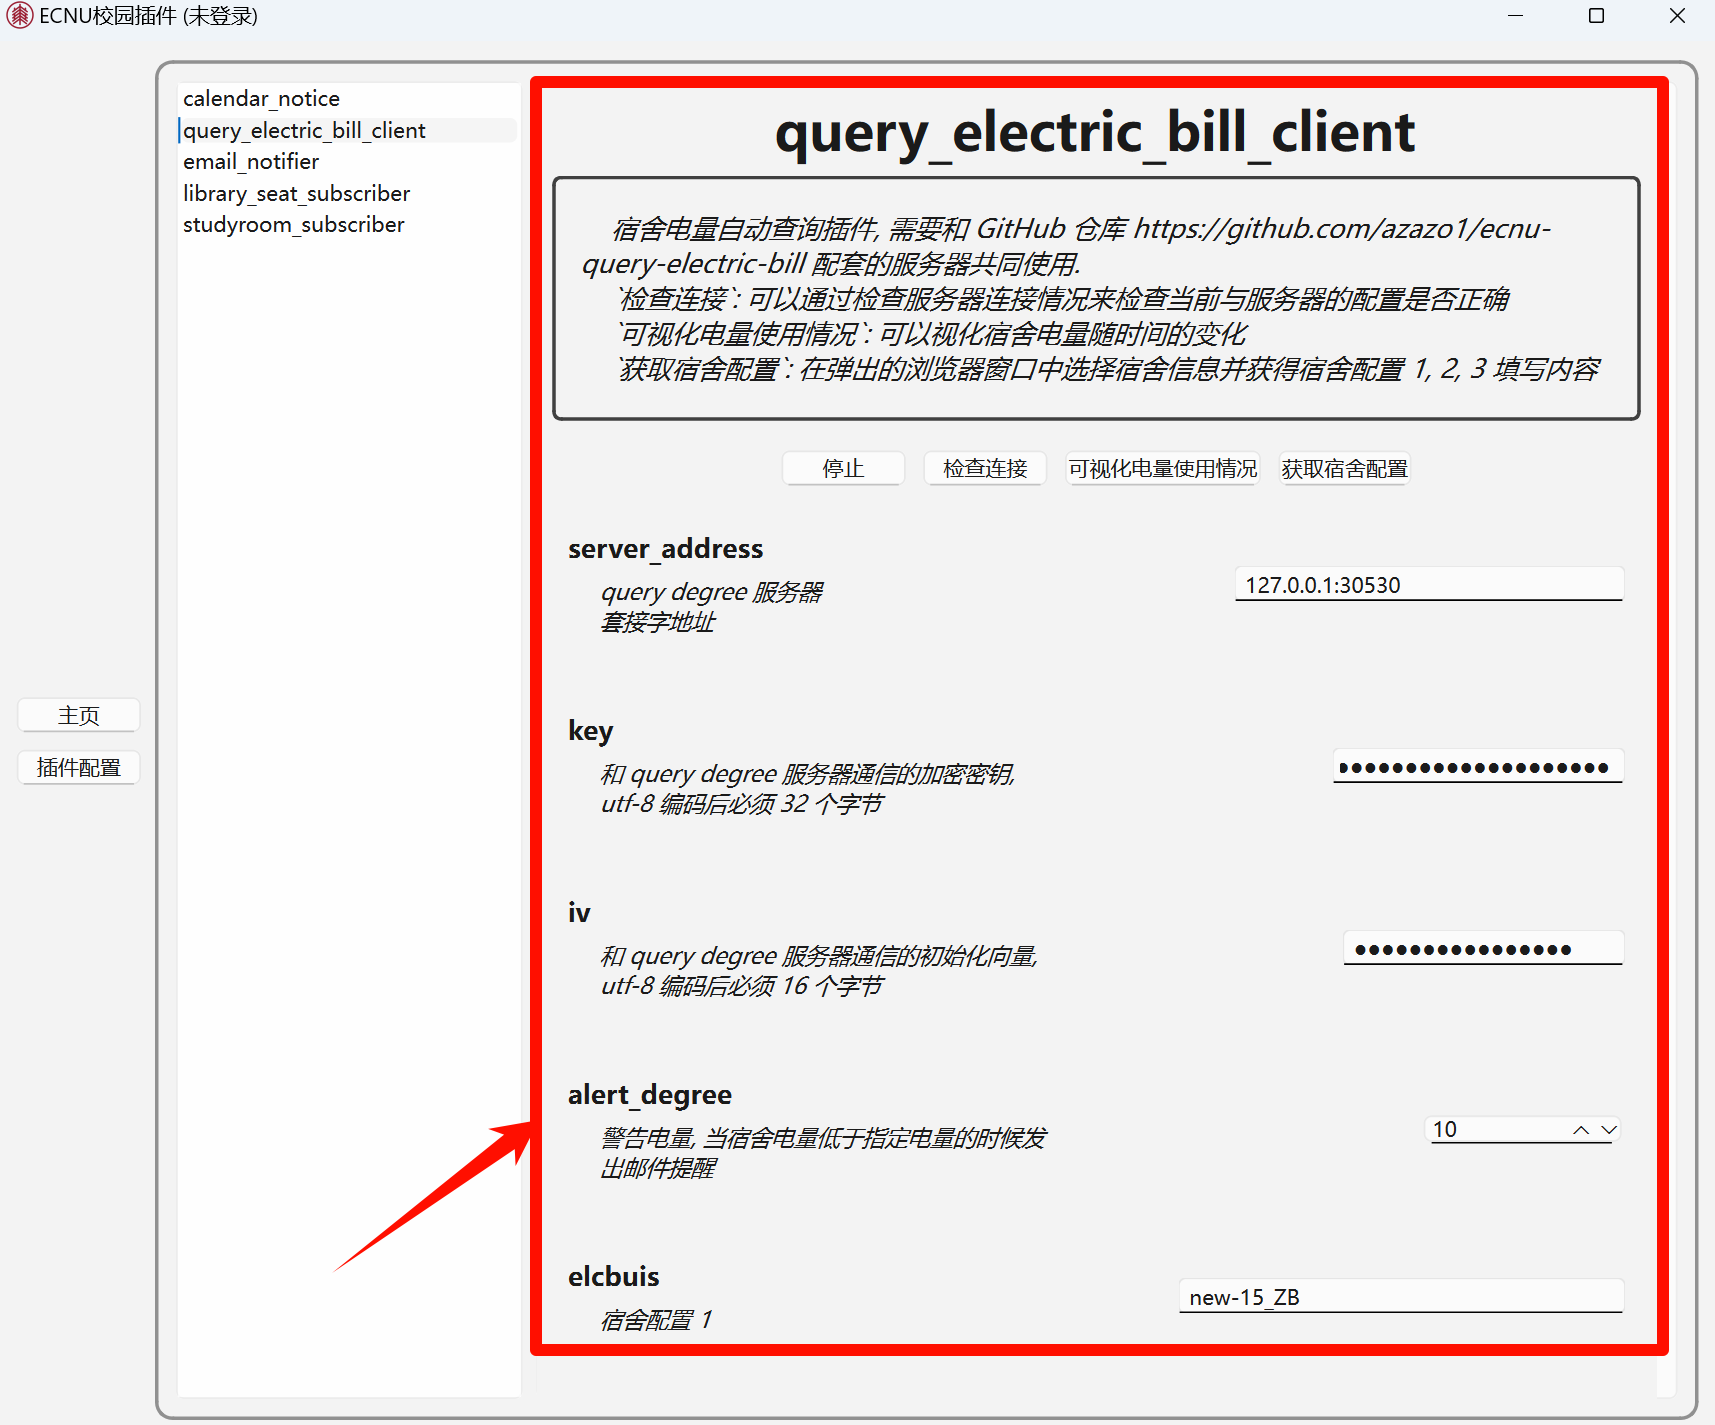
\includegraphics[width=0.6\textwidth]{img/plugin_config_gui}
    \caption{插件配置界面示例}
    \label{fig:plugin-config-gui}
\end{figure}

\newpage{}

\subsection{系统托盘图标}

启动项目后,托盘中会出现 ECNU 的图标,鼠标悬停于其上时,可查看当前的登录状态,使用鼠标右键可显示菜单。

见图\ \ref{fig:tray-icon}、图\ \ref{fig:tray-icon-hover}、图\ \ref{fig:tray-icon-menu}。

\begin{figure}[H]
    \centering
    \begin{subfigure}[H]{0.3\textwidth}
        \centering
        
\includegraphics[width=0.3\textwidth]{img/tray_icon}
        \caption{系统托盘图标}
        \label{fig:tray-icon}
    \end{subfigure}
    \begin{subfigure}[H]{0.3\textwidth}
        \centering
        
\includegraphics[width=0.48\textwidth]{img/tray_icon_hover}
        \caption{鼠标悬浮显示状态}
        \label{fig:tray-icon-hover}
    \end{subfigure}
    \begin{subfigure}[H]{0.3\textwidth}
        \centering
        
\includegraphics[width=0.6\textwidth]{img/tray_icon_menu}
        \caption{右键显示菜单}
        \label{fig:tray-icon-menu}
    \end{subfigure}
\end{figure}

\section{总结}

\subsection{项目前景}

由于本项目具备良好的扩展性,后续可以集成更多插件,覆盖更多校园生活场景。例如:

\begin{itemize}
    \item 支持课表与日历软件(如 Google Calendar)的无缝同步。
    \item 集成更多校园生活服务,例如自动化导出成绩单、图书馆借阅管理、校园卡消费查询等。
\end{itemize}

通过持续迭代和优化,本项目有潜力为华东师范大学的师生带来更加便利的校园生活体验。

\subsection{项目收获}

\subsubsection*{关卓谦}

\begin{Thought}
在本项目中, 我主要负责代码的编写.
我设计并实现了可扩展的插件架构, 支持插件的动态加载与停止, 并实现了插件数据的独立管理.
我还使用 PySide6 设计了界面布局, 事件交互逻辑, 与插件系统的无缝集成.
项目中的电费查询插件, 图书馆座位预约插件也是我编写的.

通过此次项目的实践, 尝试编写高可拓展性的代码, 我更加深入地感受到了 python 代码的灵活性;
我也借此机会将校园生活中的信息数据与代码相结合, 感受到了校园网站开发者的辛勤劳动;
我得以熟悉 Qt 框架的大致使用方法;
在和其他参与者进行交流和开发的时候, 我也认识到了应该如何去规范地进行版本控制, 代码管理, 解决团队中不一致的观点.

这些经验都会为我以后的学习生活提供有效帮助.
\end{Thought}

\subsubsection*{张梓卫}

\begin{Thought}
得益于良好的团队框架,后来使用团队中完善的 \texttt{Cache\_grabber} 框架,
让我能够马上上手研修间预约模块的开发,熟悉了数据处理和 API 调用的结合应用,
当然,LateX 课表生成器的开发让我对编译有了更深入的理解,

\vspace{0.3cm}

在不断翻看关卓谦的 \texttt{PluginLoader} 的代码到理解,最终写出一份详解的报告
从提出到实现,从实现到推翻重来,一切都有迹可循。
通过团队交流,我增强了自己的跨领域的开发编程能力,掌握了 Git 多种不同的使用方式,
同时跟随团队的项目规范,掌握了如何通过良好的代码架构提高代码复用性和维护性。

\vspace{0.3cm}

同时,我还学到了如何利用 Python 的自动化工具(Selenium-Wire 和 requests)
实现复杂的登录流程。翻看华东师范大学开发者文档时,涉及到鉴权,还了解到了 OAuth 2.0 和 JWT 等的认证机制。

\vspace{0.3cm}

是非常愉悦的一次项目经历!
\end{Thought}

\subsubsection*{王文锦}

\begin{Thought}
在本项目中
\end{Thought}

\end{document}